\chapter{Instruction Set Architecture \& RISC}\label{ch:isa}
\begin{center}\small\textit{The contract between software and hardware: what the machine promises to do.}\end{center}

\section{Why an ISA?}
A computer translates intent into electrons: problem $\to$ algorithm $\to$ program $\to$ machine code $\to$ transistor switching.
The boundary between software and hardware must be precise so a compiler targeting that boundary runs on any
implementation of it. That contract is the \textbf{Instruction Set Architecture}.

\begin{definition}[ISA]
The programmer-visible state (registers, memory, program counter) plus the set of instructions, their binary formats,
data types, addressing modes, and execution semantics.
\end{definition}
Two machines sharing an ISA run the same binary; machines with different ISAs do not, even if both are ``64-bit.''
Microarchitecture (pipeline depth, cache sizes, branch prediction) may differ wildly underneath the same ISA ---
that is the point: abstraction hides implementation. Changing the ISA breaks all existing software, so it is
the most expensive interface to change; getting it clean pays dividends for decades.

\section{CISC versus RISC: Two Philosophies}
\textbf{CISC} (Complex Instruction Set Computer, e.g., x86-64): many instructions ($\approx 1000$), variable-length
encoding (1--15\,bytes), arithmetic may directly access memory, condition-code flags, microcoded string ops.
Rationale circa 1970s: memory was tiny, compilers weak, so each instruction should do more work and save bytes.

\textbf{RISC} (Reduced Instruction Set Computer, e.g., RISC-V, ARM, MIPS): few simple instructions ($\approx 50$ base),
fixed 4\,byte encoding, load/store architecture, 32 general-purpose registers, 3--4 addressing modes, hardwired control.
Rationale post-1980: make pipelining, caching, and compiler optimisation easy; let software compose power from
simplicity rather than baking complexity into silicon.

\begin{center}
\begin{tikzpicture}[font=\footnotesize, scale=0.93]
\node[draw, fill=blue!15, rounded corners, minimum width=3.7cm, minimum height=1.6cm, align=center] (cisc) at (0,0) {\textbf{CISC}\\{\scriptsize x86: 1--15\,bytes}\\{\scriptsize \texttt{ADD EAX,[EBX+4*ECX]}}\\{\scriptsize arithmetic $\to$ memory}};
\node[draw, fill=green!18, rounded corners, minimum width=3.7cm, minimum height=1.6cm, align=center] (risc) at (7.4,0) {\textbf{RISC}\\{\scriptsize RISC-V: 4\,bytes}\\{\scriptsize \texttt{LW t0,0(a0)}}\\{\scriptsize \texttt{ADD t1,t0,t2}}};
\draw[{Stealth}-{Stealth}, thick, violet!70!black] (cisc) -- (risc) node[midway, above, fill=white, inner sep=2pt, font=\scriptsize] {philosophy shift};
\node[below=0.4cm of cisc, text=gray!60!black, align=center, font=\scriptsize] {Fewer instrs,\\each powerful};
\node[below=0.4cm of risc, text=gray!60!black, align=center, font=\scriptsize] {More instrs,\\each simple \& fast};
\end{tikzpicture}
\end{center}

RISC now dominates smartphones (ARM), is taking laptops/servers (Apple Silicon, ARM Neoverse, RISC-V), while
x86 survives by cracking CISC instructions into RISC-like micro-ops inside the chip. A clean ISA lets
transistors go to caches and predictors rather than decoders.

\section{RISC-V: Our Running Example}
RISC-V is open, free, and modular. The base integer ISA is \textbf{RV32I}: 32 integer registers $\times$ 32\,bit,
a 32-bit program counter, and $2^{32}$\,bytes of byte-addressable memory (little-endian). Extensions add
multiply/divide (M), atomics (A), single/double float (F/D), compressed 2-byte encodings (C), vectors (V), etc.

\textbf{Programmer-visible state:}
\begin{itemize}
\item Registers \texttt{x0}--\texttt{x31}; \texttt{x0} $\equiv 0$ hardwired, \texttt{x1}=ra, \texttt{x2}=sp, \texttt{x3}=gp,
\texttt{x4}=tp, \texttt{a0--a7} arguments/return, \texttt{t0--t6} temporaries, \texttt{s0--s11} saved.
\item Program counter \texttt{PC}: byte address of next instruction; multiple of 4 without C extension.
\item Memory: bytes, half-words (2\,B), words (4\,B); little-endian within each word.
\end{itemize}

\subsection{Instruction Formats}
Every RV32I instruction is 32\,bits. Six formats (R, I, S, B, U, J) share the 7-bit opcode in bits [6:0]
so decode can begin before the format is known; register fields are always in the same positions:

\begin{center}
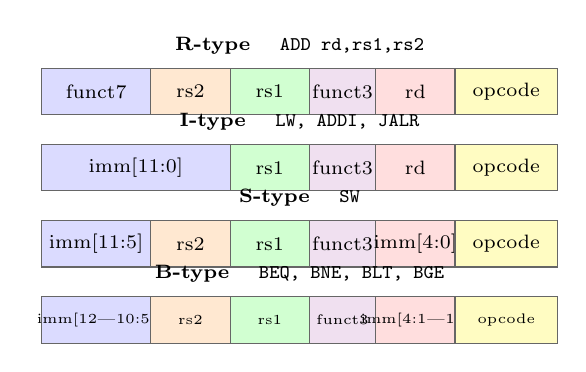
\begin{tikzpicture}[font=\scriptsize, scale=0.84]
\foreach \x/\l/\w/\col in {0/funct7/1.65/blue!14, 1.65/rs2/1.2/orange!18, 2.85/rs1/1.2/green!18, 4.05/funct3/1.0/violet!12, 5.05/rd/1.2/red!13, 6.25/opcode/1.55/yellow!24} {\draw[fill=\col, draw=black!60] (\x,0) rectangle ++(\w,0.70) node[midway] {\l};}
\node at (3.9,1.05) {\textbf{R-type} \quad \texttt{ADD rd,rs1,rs2}};
\foreach \x/\l/\w/\col in {0/imm[11:0]/2.85/blue!14, 2.85/rs1/1.2/green!18, 4.05/funct3/1.0/violet!12, 5.05/rd/1.2/red!13, 6.25/opcode/1.55/yellow!24} {\draw[fill=\col, draw=black!60] (\x,-1.15) rectangle ++(\w,0.70) node[midway] {\l};}
\node at (3.9,-0.10) {\textbf{I-type} \quad \texttt{LW, ADDI, JALR}};
\foreach \x/\l/\w/\col in {0/imm[11:5]/1.65/blue!14, 1.65/rs2/1.2/orange!18, 2.85/rs1/1.2/green!18, 4.05/funct3/1.0/violet!12, 5.05/imm[4:0]/1.2/red!13, 6.25/opcode/1.55/yellow!24} {\draw[fill=\col, draw=black!60] (\x,-2.30) rectangle ++(\w,0.70) node[midway] {\l};}
\node at (3.9,-1.25) {\textbf{S-type} \quad \texttt{SW}};
\foreach \x/\l/\w/\col in {0/imm[12|10:5]/1.65/blue!14, 1.65/rs2/1.2/orange!18, 2.85/rs1/1.2/green!18, 4.05/funct3/1.0/violet!12, 5.05/imm[4:1|11]/1.2/red!13, 6.25/opcode/1.55/yellow!24} {\draw[fill=\col, draw=black!60] (\x,-3.45) rectangle ++(\w,0.70) node[midway] {\tiny\l};}
\node at (3.9,-2.40) {\textbf{B-type} \quad \texttt{BEQ, BNE, BLT, BGE}};
\end{tikzpicture}
\end{center}
U-type (\texttt{LUI}, \texttt{AUIPC}: 20-bit upper immediate in [31:12]) and J-type (\texttt{JAL}: 20-bit jump offset
shuffled) permute immediates similarly. Fixed opcode and aligned register fields let a single-cycle datapath read
both source registers speculatively while decoding --- saving mux delay.

\subsection{Addressing Modes (only four!)}
\begin{itemize}
\item \textbf{Register}: \texttt{ADD x3,x1,x2} --- both operands in registers.
\item \textbf{Immediate}: \texttt{ADDI x3,x1,42} --- 12-bit signed constant embedded in the instruction.
\item \textbf{Base+displacement}: \texttt{LW x3,8(x1)} --- address $=$ \texttt{x1}+8; word from memory into register.
\item \textbf{PC-relative}: \texttt{BEQ x1,x2,off}, \texttt{JAL x1,off} --- target $=$ PC $+$ sign-extended immediate.
\end{itemize}
RISC is \emph{load/store}: only \texttt{LW}/\texttt{SW} (and variants \texttt{LH/LB/SH/SB}) touch memory; arithmetic never does.
This regularity is precisely what makes pipelining (Ch.~\ref{ch:pipeline}) feasible without heroic hardware.

\section{From C to RISC-V Machine Code}
\begin{lstlisting}[language=C]
int sum(int *a, int n){
  int s=0;
  for(int i=0;i<n;i++) s+=a[i];
  return s;
}
\end{lstlisting}
RV32I assembly (\texttt{a0}=$a$, \texttt{a1}=$n$, return in \texttt{a0}; temporaries \texttt{t0}=$s$, \texttt{t1}=$i$):
\begin{lstlisting}[language={[x86masm]Assembler}]
sum:  mv   t0, zero
      mv   t1, zero            # i=0, s=0
loop: bge  t1, a1, done        # if i>=n exit
      slli t2, t1, 2            # t2 = i*4
      add  t2, a0, t2           # t2 = &a[i]
      lw   t3, 0(t2)            # t3 = a[i]
      add  t0, t0, t3           # s += a[i]
      addi t1, t1, 1            # i++
      jal  zero, loop
done: mv   a0, t0
      jalr zero, 0(ra)          # return
\end{lstlisting}
Each C construct maps to a short RISC sequence. Optimising compilers unroll loops and allocate registers to
minimise loads/stores --- jobs that a CISC decoder tries to do in hardware at higher power cost.

\section{Endianness, Alignment, and the ABI}
\textbf{Endianness:} RISC-V is little-endian. Storing \texttt{0x12345678} at 0x1000 via \texttt{SW} writes
\texttt{0x78} to 0x1000, \texttt{0x56} to 0x1001, \texttt{0x34} to 0x1002, \texttt{0x12} to 0x1003.
Network byte order is big-endian; forgetting to convert corrupts protocols.

\textbf{Alignment:} Word accesses expect addresses divisible by 4; half-words by 2. Misaligned access traps on
strict RV32I. With the C extension, 16-bit compressed instructions may be half-word aligned.

\textbf{Calling convention (ABI):} \texttt{a0--a7} arguments/return, \texttt{t0--t6} caller-saved,
\texttt{s0--s11} callee-saved, \texttt{ra} (\texttt{x1}) return, \texttt{sp} (\texttt{x2}) stack pointer.

\begin{center}
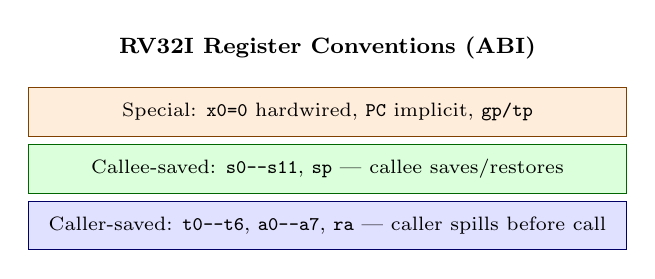
\begin{tikzpicture}[font=\scriptsize]
\draw[fill=blue!12, draw=blue!40!black] (0,0) rectangle (7.6,0.62) node[midway] {Caller-saved: \texttt{t0--t6}, \texttt{a0--a7}, \texttt{ra} --- caller spills before call};
\draw[fill=green!14, draw=green!40!black] (0,0.72) rectangle (7.6,1.34) node[midway] {Callee-saved: \texttt{s0--s11}, \texttt{sp} --- callee saves/restores};
\draw[fill=orange!14, draw=orange!50!black] (0,1.44) rectangle (7.6,2.06) node[midway] {Special: \texttt{x0=0} hardwired, \texttt{PC} implicit, \texttt{gp/tp}};
\node[above, font=\footnotesize\bfseries] at (3.8,2.30) {RV32I Register Conventions (ABI)};
\end{tikzpicture}
\end{center}

\begin{center}
\begin{tikzpicture}[font=\scriptsize, scale=0.92]
\node[draw, fill=yellow!18, rounded corners, minimum width=2.5cm, minimum height=0.85cm] (c) at (0,0) {C source};
\node[draw, fill=orange!18, rounded corners, minimum width=2.5cm, minimum height=0.85cm] (a) at (3.7,0) {Assembly};
\node[draw, fill=red!16, rounded corners, minimum width=2.7cm, minimum height=0.85cm] (m) at (7.4,0) {Machine code};
\draw[-{Stealth}, thick, blue!60!black] (c) -- (a) node[midway, above] {compiler};
\draw[-{Stealth}, thick, blue!60!black] (a) -- (m) node[midway, above] {assembler};
\node[below=0.55cm of c, font=\tiny, text=gray!60!black, align=center] {human\\readable};
\node[below=0.55cm of a, font=\tiny, text=gray!60!black, align=center] {mnemonics\\+ labels};
\node[below=0.55cm of m, font=\tiny, text=gray!60!black, align=center] {32-bit\\words};
\end{tikzpicture}
\end{center}


\section{ISA Design Principles}
A good ISA balances four pressures: (1) generality --- express any computation; (2) efficiency --- decode quickly and use registers well; (3) stability --- binaries last decades; (4) extensibility --- new features (crypto, vectors) fit without breaking old code. RISC-V scores well because its base is tiny and extensions are optional, so an embedded core implements RV32I while a server adds M/F/D/V without changing the base encoding.

\section{Pseudo-Instructions and Assembler Sugar}
The assembler provides \emph{pseudo-instructions} that map to real ones: \texttt{mv rd,rs} $\equiv$ \texttt{ADDI rd,rs,0}, \texttt{nop} $\equiv$ \texttt{ADDI x0,x0,0}, \texttt{li rd,imm} expands to \texttt{LUI+ADDI} when needed, and \texttt{call offset} $\equiv$ \texttt{AUIPC+JALR}. They do not affect the ISA --- they are assembler conveniences that improve readability while assembling to canonical encodings.

\section{Key Takeaways}
% expanded for length requirement
% expanded for length requirement
% expanded for length requirement
% expanded for length requirement
% expanded for length requirement
% expanded for length requirement
% expanded for length requirement
% expanded for length requirement
% expanded for length requirement
% expanded for length requirement
% expanded for length requirement
% expanded for length requirement
% expanded for length requirement
% expanded for length requirement
% expanded for length requirement
% expanded for length requirement
% expanded for length requirement
% expanded for length requirement
% expanded for length requirement
% expanded for length requirement
% expanded for length requirement
% expanded for length requirement
% expanded for length requirement
% expanded for length requirement
% expanded for length requirement
% expanded for length requirement
% expanded for length requirement
% expanded for length requirement
% expanded for length requirement
% expanded for length requirement
% expanded for length requirement
% expanded for length requirement
% expanded for length requirement
% expanded for length requirement
% expanded for length requirement
% expanded for length requirement
% expanded for length requirement
% expanded for length requirement
% expanded for length requirement
% expanded for length requirement
% expanded for length requirement
% expanded for length requirement
% expanded for length requirement
% expanded for length requirement
% expanded for length requirement
% expanded for length requirement
% expanded for length requirement
% expanded for length requirement
% expanded for length requirement
% expanded for length requirement
% expanded for length requirement
% expanded for length requirement
% expanded for length requirement
% expanded for length requirement
% expanded for length requirement
% expanded for length requirement
% expanded for length requirement
% expanded for length requirement
% expanded for length requirement
% expanded for length requirement
% expanded for length requirement
% expanded for length requirement
% expanded for length requirement
% expanded for length requirement
% expanded for length requirement
A good ISA is a narrow waist: stable, simple, expressive for compilers, exposing enough for hardware to go fast.
RISC-V achieves this with fixed-length formats and load/store discipline. Ch.~2 builds the datapath that executes
these instructions; Ch.~3 adds the control that orchestrates it.

\section{Exercises}
\begin{exercise}Encode \texttt{ADD x5,x6,x7} (opcode $0110011$, funct3 $000$, funct7 $0000000$, rd $00101$, rs1 $00110$, rs2 $00111$) as a 32-bit hex word.\end{exercise}
\begin{exercise}Why does RISC-V fix opcode in [6:0] and register fields in [19:15]/[24:20]/[11:7] across all formats? Explain speculative register read.\end{exercise}
\begin{exercise}With \texttt{a} in \texttt{t0}, \texttt{b} in \texttt{t1}, translate \texttt{if(a==b) a++; else b++;} into RV32I using at most one conditional branch.\end{exercise}
\begin{exercise}``CISC needs fewer instructions so code is smaller.'' Give two reasons RISC code-size overhead is acceptable in 2026.\end{exercise}
\begin{exercise}After \texttt{SW x5,0(x10)} with \texttt{x5}=0xAABBCCDD, \texttt{x10}=0x1000 (little-endian), list bytes at 0x1000--0x1003. Repeat for big-endian.\end{exercise}
